\documentclass{sig-alternate}
\usepackage{graphicx, subfigure, multirow, times, balance}
\usepackage{url, amsfonts, verbatim, mathtools}

\renewcommand{\ttdefault}{cmtt}
\usepackage{mdwlist}

\newenvironment{myitemize}
{
   \vspace{0mm}
    \begin{list}{$\bullet$ }{}
        \setlength{\topsep}{0em}
        \setlength{\parskip}{0pt}
        \setlength{\partopsep}{0pt}
        \setlength{\parsep}{0pt}         
        \setlength{\itemsep}{1mm} 
}
{
    \end{list} 
    \vspace{-1em}
}

\newcommand{\vignette}[1]{\textit{\\[-.5em]\noindent#1\\[-.5em]}}

\begin{document}

\title{PBS at Work: Advancing Data Store Operation via Consistency Metrics}

\author{Peter Bailis, Shivaram Venkataraman, Michael J. Franklin, Joseph M. Hellerstein, Ion Stoica\\
\affaddr{University of California, Berkeley}\\
\affaddr{\{pbailis, shivaram, franklin, hellerstein, istoica\}@cs.berkeley.edu}}

\interfootnotelinepenalty=10000
\hyphenation{prob-a-bil-is-tic-ally}
\hyphenation{exchan-ged}

\maketitle

\begin{abstract}
A large body of recent work has proposed analytical and empirical
techniques for quantifying the data consistency properties of
distributed data stores. In this demonstration, we begin to explore
the wide range of new database functionality they enable, including
dynamic query tuning, consistency SLAs, monitoring, and
administration. Our demonstration will exhibit how both application
programmers and database administrators can leverage these features.
We describe three major application scenarios and present a system
architecture for supporting them. We also describe our experience in
integrating Probabilistically Bounded Staleness (PBS) predictions into
Cassandra, a popular NoSQL store and sketch a demonstration that will
allow SIGMOD attendees to experience the importance and applicability
of real-time consistency metrics.
\end{abstract}

\section{Introduction}

Modern distributed data stores offer a choice. Weak consistency models
are fast and guarantee ``always-on'' behavior, but provide limited
semantics. Stronger consistency models are easier to reason about but
slower and potentially unavailable. The choice of consistency has
wide-ranging implications for application writers, operations
management, and end-users, and, in light of its performance benefits,
weak consistency is often acceptable.

Using one predominant consistency model, eventual consistency, is, on
its face, a cavalier proposition. Prevalent models such as eventual
consistency provide no guarantees as to when new writes will become
visible to readers and what versions of data items will be presented
in the interim. Reading all \texttt{null} values from a database is
eventually consistent. The data store can delay write visbility for
decades and not violate its guarantees. Yet, despite these weak
semantics, there is common sentiment among practitioners that eventual
consistency is often ``good enough'' and ``worthwhile'' for many
applications.

In recent work, we provided an analytical and empirical framework for
analyzing the consistency provided by eventually consistent stores, or
``how eventual and how consistent is eventual consistency?'', called
Probabilistically Bounded Staleness, or PBS. Eventually consistent
stores do not make promises about answers to the length of time
required to observe an update or the staleness of values, but this
does not preclude us from making informed statements about what is
likely to happen. By using expert knowledge of the underlying data
store and its replication protocols in addition to some lightweight
in-situ profiling, we can inform data store users about what
consistency they are likely to observe in the future.

Our PBS predictions are part of a larger trend towards providing
quantitative measurements and analysis of weakly consistent
stores. There is recent work ranging from distributed systems theory
to database practitioner communities on measuring violations of
properties such as atomicity, serializability, and regular register
semantics. PBS in particular has experienced relative popularity in
the NoSQL community and our implementation of PBS for quorum-based
systems was recently accepted to Cassandra's mainline source trunk and
will be released by the end of 2012. Afeter discussions with other
researchers pursuing consistency monitoring and verification, we
expect more technology transfer in this space.

While monitoring and prediction are useful in themselves, perhaps more
importantly, they enable a rich space of applications that we believe
have been neglected. For example, in our initial PBS work, we mostly
assume that simply recording the predictions is a worthwhile task:
what they are used for is mostly left for future work. We are most
excited about three particular applications: \textit{i.)} dynamic
request-based consistency parameters, or auto-tuning request routing
based on a given latency and consistency service level agreement,
\textit{ii.)} database administration tasks with respect to the impact
of slow nodes and networks, replication factors, and data store
paramers like anti-entropy rates, and \textit{iii.)} integration into
traditional alerts and monitoring frameworks. We elaborate further in
Section~\ref{sec:scenarios}, but, in short, these quantitative metrics
allow new ways to tune the performance, semantics, and the maintenance
of eventually consistent stores.

In this demo proposal, we outline these advanced use cases in detail
(Section~\ref{sec:scenarios}), describe how both quantitative metrics
can be integrated into existing stores and architectures based on our
experiences with the Cassandra community
(Section~\ref{sec:architecture}), and sketch how we plan to
demonstrate this newly enabled functionality, allowing SIGMOD
attendees to act as both end-users and operations managers for an
eventually consistent service (Section~\ref{sec:demo}).

\section{Usage Scenarios}
\label{sec:scenarios}

Quantitative consistency metrics are useful for a variety of services
that can tolerate eventual consistency. In this section, we outline
three use cases in the context of a hypothetical microblogging web
service, Twissistency.

\subsection{Dynamic Reconfiguration}
\label{sec:dynamic}

Without quantitative guidance, choosing the correct values for
replication parameters is a difficult task. We believe that, instead
of reasoning about low-level replication settings, application writes
should instead declaratively specify their objectives in the form of
higher-level service agreements and allow the system to adjust its
parameters to meet this goal.\\

Data stores often offer a choice between replication parameters. For
example, in Dynamo-style sytems like Cassandra, applications can
choose the minimum number of replicas to read from ($R$) and write to
($W$). If $R$+$W$ is greater than the number of replicas ($N$),
operations will achieve \textit{strong consistency}, and, if not, the
system provides \textit{eventual consistency}. With a replication
factor of $N=3$, we have three options for eventually consistent
operation: $R$$=$$W$$=$$1$, $R$$=$$1$$, W$$=$$2$, and $R$$=$$2$$,
W$$=$$1$.  $R$$=$$W$$=$$1$ is guaranteed to be fastest, but it is also
the least consistent. Instead of thinking about $R$ and $W$, the
developers can think in terms of desired $t$-visibility:

\vignette{Twissistency's data scientists have learned that their users
  respond negatively to slow update propagation, and the company sets
  a $t$-visibility target of 500ms at the 99.9th percentile for their
  back-end data store requests (while minimizing latency).}

How should we configure the replication parameters for a given SLA?
One approach is to manually tune the system---this is straightforward
but is not necessarily robust to changing conditions:

\vignette{Based on feedback from their infrastructure team, the
  developers set $R$=$W$=$1$ for their Dynamo-based data store. This
  meets the $t$-visibility consistency SLA, but, during peak traffic,
  the consistency SLA is sporadically violated.}

Instead, we can auto-tune the replication parameters for each
request. Consistency monitoring allows us to monitor SLA violations,
while consistency prediction allows us the system to do forward testing of
replication parameter changes before making them:

\vignette{The consistency autotuner uses R=W=1 for most traffic but
  switches to R=2, W=1 during peak workload times. While R=1, W=2 is
  also a viable solution, the autotuner determines that the 99.9th
  percentile operation latency would suffer since most reads are
  served from the data store's buffer cache.}

While the literature suggests several dynamic replication
schemes~\cite{vahdat-article}, we are pleased that these
techniques are now a reality for production-ready data stores.

\subsection{DBA Integration}
\label{sec:dba}

Consistency metrics can also be used in diagnostic tasks and to
understand \textit{why} a system is misbehaving. There are a number of
system parameters which affect the performance and observed
consistency of a distributed data store. System administrators
currently face two major feature shortcomings: limited
information available in terms of the currently observed consistency
properties and lack of easy methods to understand how the
system will behave as parameters are varied.

\vignette{The database administrators at Twissistency have received
  reports that a high-profile user is seeing very stale data.}

There are a host of consistency configuration options available to
data store administrators. Taking Cassandra as an example, the administrators can
configure read repair rates, perform active anti-entropy value
exchange, and enable or disable replicas. Moreover, there are many
causes for inconsistent reads: there may be slow nodes in the cluster
or that there are some keys which are hotspots.

\vignette{The administrators inspect the consistency metrics for each
  data store shard and identify a misbehaving set of nodes
  corresponding to a bad top-of-rack switch. They temporarily increase
  the rate of background version exchange for the shard and begin to
  spin up a new replica set on a different rack before rebooting the
  switch.}

We believe consistency metrics should allow standard analytics such as
fine-grained drill-downs and roll-ups across both logical data items
and physical-layer details like placement and hardware details. If, as
in our Cassandra implementation (Section~\ref{sec:architecture}),
monitoring is performed as a white-box, in-database service, low-level
details like network topologies and per-operation latencies will be
available to the administrator. Of course, it may be sufficient for most
operations to simply experiment with common configuration parameters via
prediction, but exposing such advanced analytics functionality is
likely useful for power users.

\subsection{Monitoring and Alerts}
\label{sec:monitoring}

Consistency metrics allow us to look at new approaches to traditional monitoring:

\vignette{Twissistency has a large number of DevOps who are
  responsible for keeping their service up and running. Currently
  their monitoring and pager service is triggered when operation
  latency is high or if servers fail. As user experience is negatively
  impacted by inconsistent reads, the CTO wants to ensure that DevOps
  respond to these alerts.}

As we discussed in Section~\ref{sec:dynamic}, some parameters like
per-request quorum settings, are amenable to SLA-based automatic
control. However, there are a number of scenarios where traditional,
manual monitor-and-respond is an acceptable approach. If SLAs cannot
be met under any circumstances (e.g., operation latency and
$t$-visibility bounds are too restrictive), the correct response is to
revise the SLAs or perform more invasive operations (e.g., add more
replicas) which may require active human oversight.

\section{System Architecture}
\label{sec:architecture}

In this section, we briefly outline an architecture for providing
consistency monitoring and verification given our experiences
implementing both for two production NoSQL stores---Cassandra and
Voldemort. The techniques used to measure PBS are applicable to any
system for which we can model the replication protocol used and
require only lightweight latency profiling in the underlying data
store. We also explain some of the design decisions we made to
simplify PBS integration and how this could be generalized to other
systems.

%Introductory paragraph explaining the system architecture. Explain that our
%approach is to make PBS a shim layer on top of existing server code. Latency
%measurements etc.

\begin{figure}
\centering
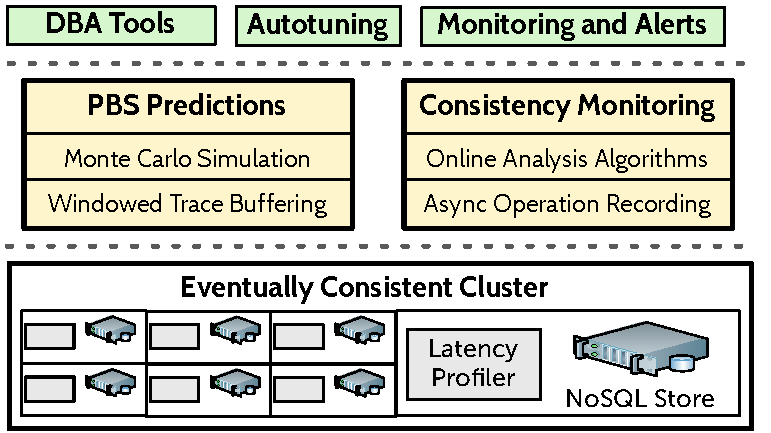
\includegraphics[width=\columnwidth]{figs/cluster-arch.pdf}
\caption{Diagram showing how PBS metrics can be integrated into an existing
NoSQL datastore. The PBS prediction module and Consistency SLA verifier drive
the metrics used the monitoring framework.}
\label{fig:pbs-sys-arch}
\end{figure}

\begin{figure*}[tb]
\centering
%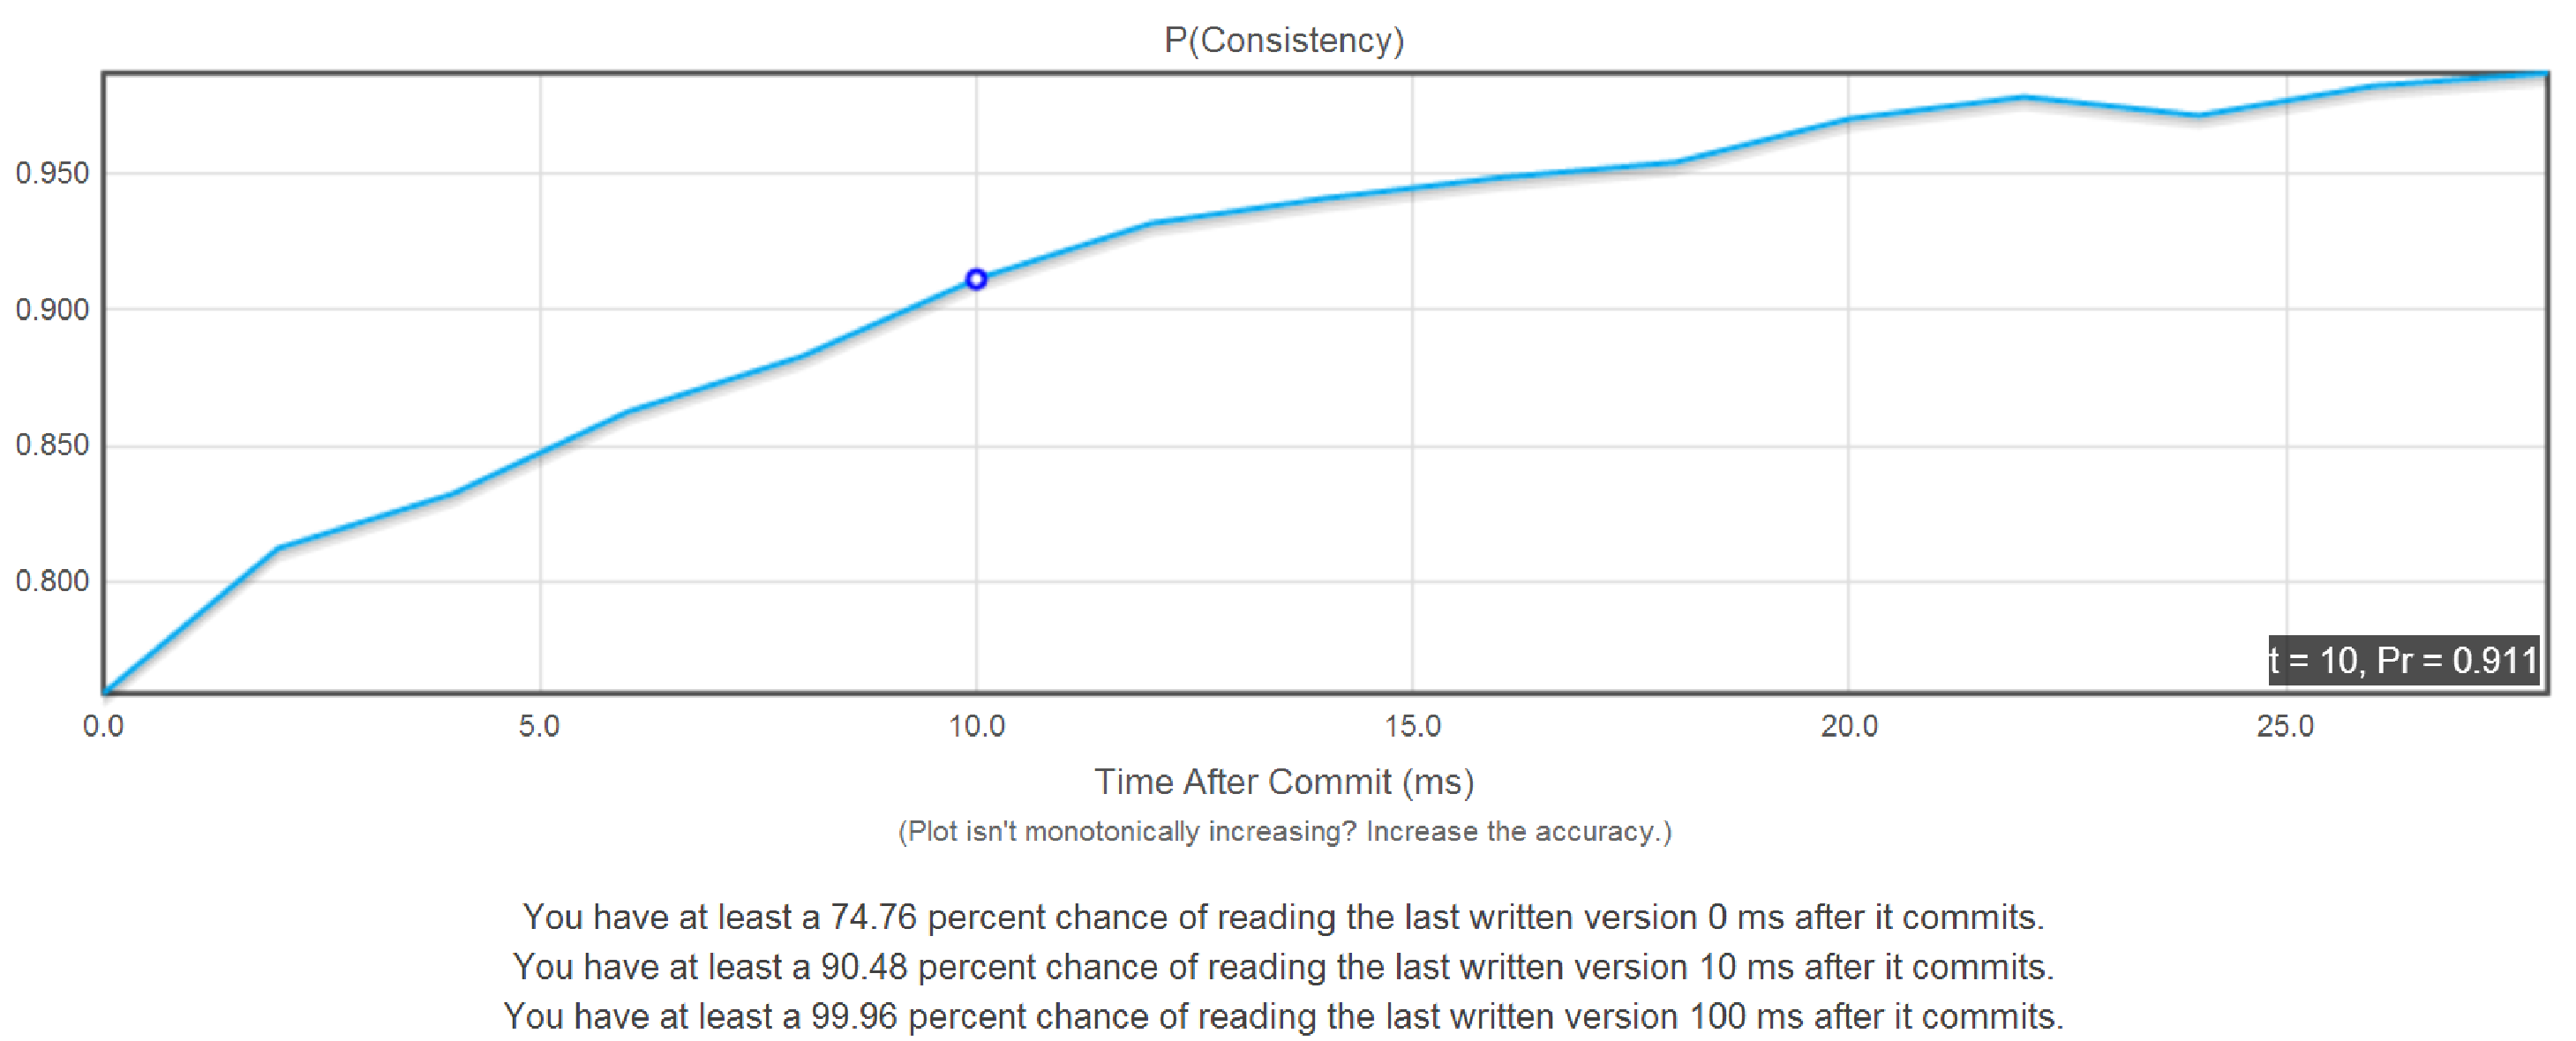
\includegraphics[width=.90\textwidth]{figs/pbs-demo-screenshot.pdf}
\subfigure[Mobile Web App]{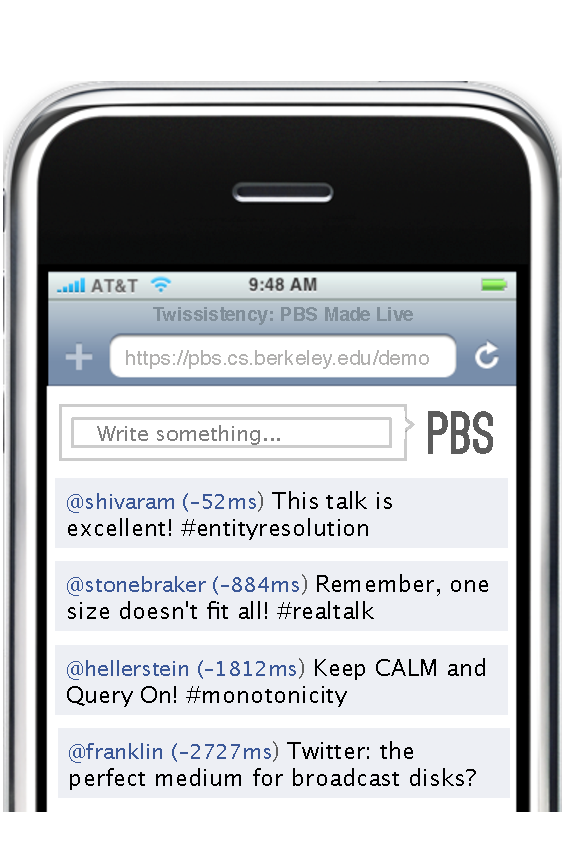
\includegraphics[width=.20\textwidth]{figs/phone.pdf}}
\subfigure[DBA and Query Tuning Dashboard]{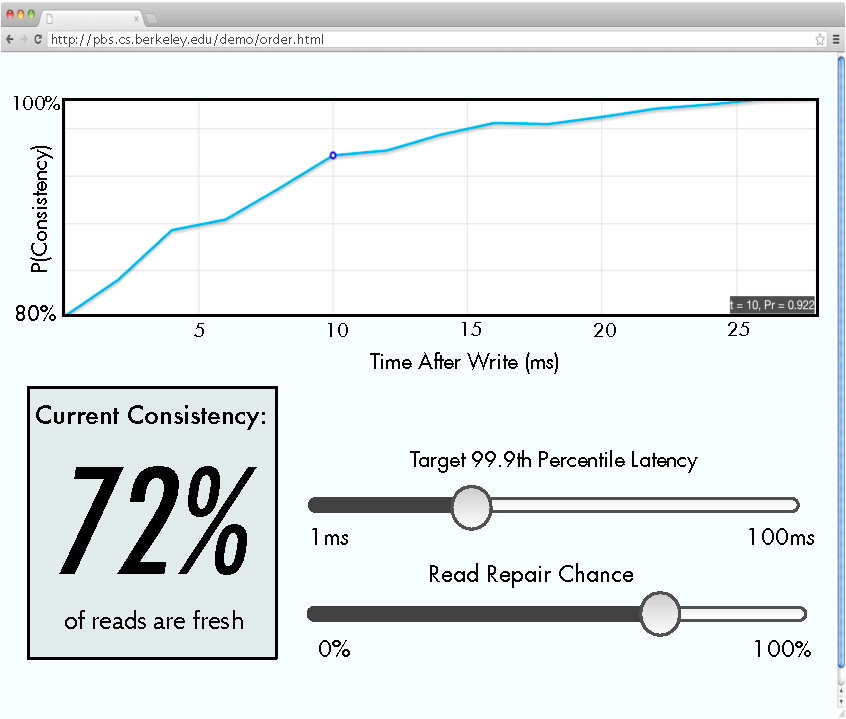
\includegraphics[width=.39\textwidth]{figs/dash.pdf}}
\subfigure[Chaos Console]{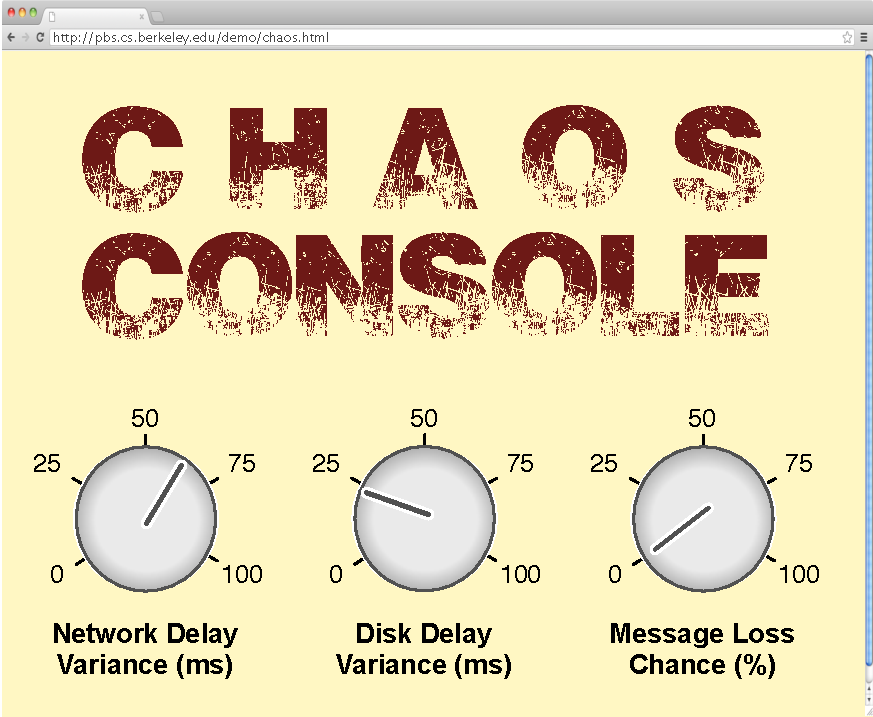
\includegraphics[width=.4\textwidth]{figs/chaos.pdf}}
\caption{Mock-ups for the mobile social web application---which
  attendees will interact with as end-users---and back-end diagnostic
  views. In the Dashboard, attendees can monitor system consistency
  and set latency and consistency SLAs. In the Chaos Console,
  attendees will wreak havoc on the application's Cassandra cluster
  via several (real-time) configurable failure modes.}
\label{fig:pbs-demo-screenshot}
\end{figure*}



\subsection{Database Architecture}

The lower half of Figure~\ref{fig:pbs-sys-arch} shows the data store
changes that are required to integrate PBS metrics into an existing
distributed database. In each replica, or storage node, we perform
lightweight latency profiling by piggybacking timestamps on messages
exchanged between servers. This data is subsequently processed by two
separate modules that provide consistency prediction and SLA
verification. These modules are cleanly separable from the main data
store implementation and can be easily adapted to different systems.\\

%Walk through the system diagram - Explain what each component does. In
%particular explain how the latency collector feeds into the PBS prediciton
%module and how the Monte-Carlo simulation can be run using this data.
\textbf{PBS Prediction:} The PBS prediction module is responsible for
calculating the $t$-visibility and $k$-staleness of the
datastore. This module is takes the latency for relevant operations in
the data store (in Dynamo-style systems, the respective latencies for
writes, acks, reads, and responses---the PBS \textit{WARS} model) that
are sent during replication.  The prediction module tracks a moving
window of recent latencies across servers, and, when an end-user (or
higher-level component) requests a consistency prediction, the module
uses the latencies to provide a prediction. Predictions are performed
using Monte Carlo analysis, and the module simulates the interactions
between thousands of read and write requests in the underlying
replication mechanism that each behave stochastically according to the
observed distributions. This allow us to estimate $t$-visibility,
$k$-staleness, and latency for the operations under a range of
parameter choices: replication factors, anti-entropy rates, and node
failures. In our Cassandra implementation, we found that the
prediction typically finishes under a second for tens of thousands of
trials.\\


%Talk about how the simulation can be triggered by either the database
%administration tool or the Consistency SLA verifier module. The consistency sla
%verifier accepts SLA specifications from clients and periodically triggers the
%prediction module - This module also completes the loop and adjusts the value of
%N,R and W until the consistency SLA is met.

\textbf{Consistency SLA verifier:} While predictions are useful, it is
also beneficial to know what consistency a data store is actually
providing. While PBS gives a precise cumulative distribution function
that reads are consistent after a fixed amount of time, consistency
verification amounts to integrating over the PDF: what percent of
reads are actually consistent? Verification is somewhat more difficult
than predictions because determining the latest write effectively
requires (background) consensus about the value of the latest
write. This requires substantially more coordination than prediction
but is the subject of considerable ongoing
research~\cite{podc-hpl}. Our verifier for Cassandra uses white-box
techniques as in the PBS predictor and the verifier collects recent
write metadata from each replica, as in the prediction step.

\subsection{Userspace tools}


As we described in Section~\ref{sec:dynamic}, one of the use cases of
consistency prediction is that the data store can use metrics to
provide SLAs on consistency. This can be accomplished by a standalone
module that tracks the consistency and latency profile of queries over
time. Database administrators can specify the SLA required in terms of
what is the maximum value of $t$-visibility, $k$-staleness, or latency
that is acceptable. The verification module periodically triggers the
PBS predictor. Based on the predictions, replication parameters are
adjusted to ensure that the SLA is met while minimizing the latency
observed. The number of possible states is limited for small values
of$ N$, so our current implementation performs a complete search over
the state space.  We have also formulated this as an integer linear
program and are exploring the use of linear solvers in the future.

%Finally talk about how the database administration tool can also trigger the pbs
%prediction. Explain how this works with respect to nodetool and the flexibility
%they have with respect to the query inteface.
The PBS predictions are not only meant to be used by automated tools
like the SLA verifier but can also be used by database administrators
to get more insights into the latency-consistency trade-offs for their
deployment. In our Cassandra implementation, we have added a new
command \texttt{predictconsistency} to \texttt{nodetool}, a widely
used administration interface.  The \texttt{predictconsistency}
command allows a flexible interface for performing PBS
prediction. Database administrators can specify the replication factor
($N$,$R$,$W$) to be used and the time at which a read is performed
after a write request. This allows administrators to perform what-if
analysis and project the impact on latency and consistency as their
workload changes.  Finally, we also export the consistency metrics
over a Java MBean interface, meaning any tool that can handle MBean
output can be used to display this data.

%Last talk a little bit about the monitoring tools and how one can export the PBS
%metrics in a time series format and alert the users if some trigger has not been
%meet for the given time period.

PBS can be used by administrators to monitor the consistency their
datastore is providing them. In contrast to offline consistency
verification schemes~\cite{podc-hpl}, PBS predictions provide a
lightweight mechanism that can be used for monitoring. A monitoring
tool like Ganglia~\cite{massie2004ganglia} or DataStax's
OpsCenter~\cite{datastax-opscenter} can be used to issue periodic PBS
prediction requests and plot the values of $t$-visibility and
$k$-staleness as a timeseries. This can then be integrated with
rule-based alerting systems to page an operator if the value of
$t$-visibility is beyond a particular threshold for an extended time
period.



\begin{figure*}[!tb]
\centering
%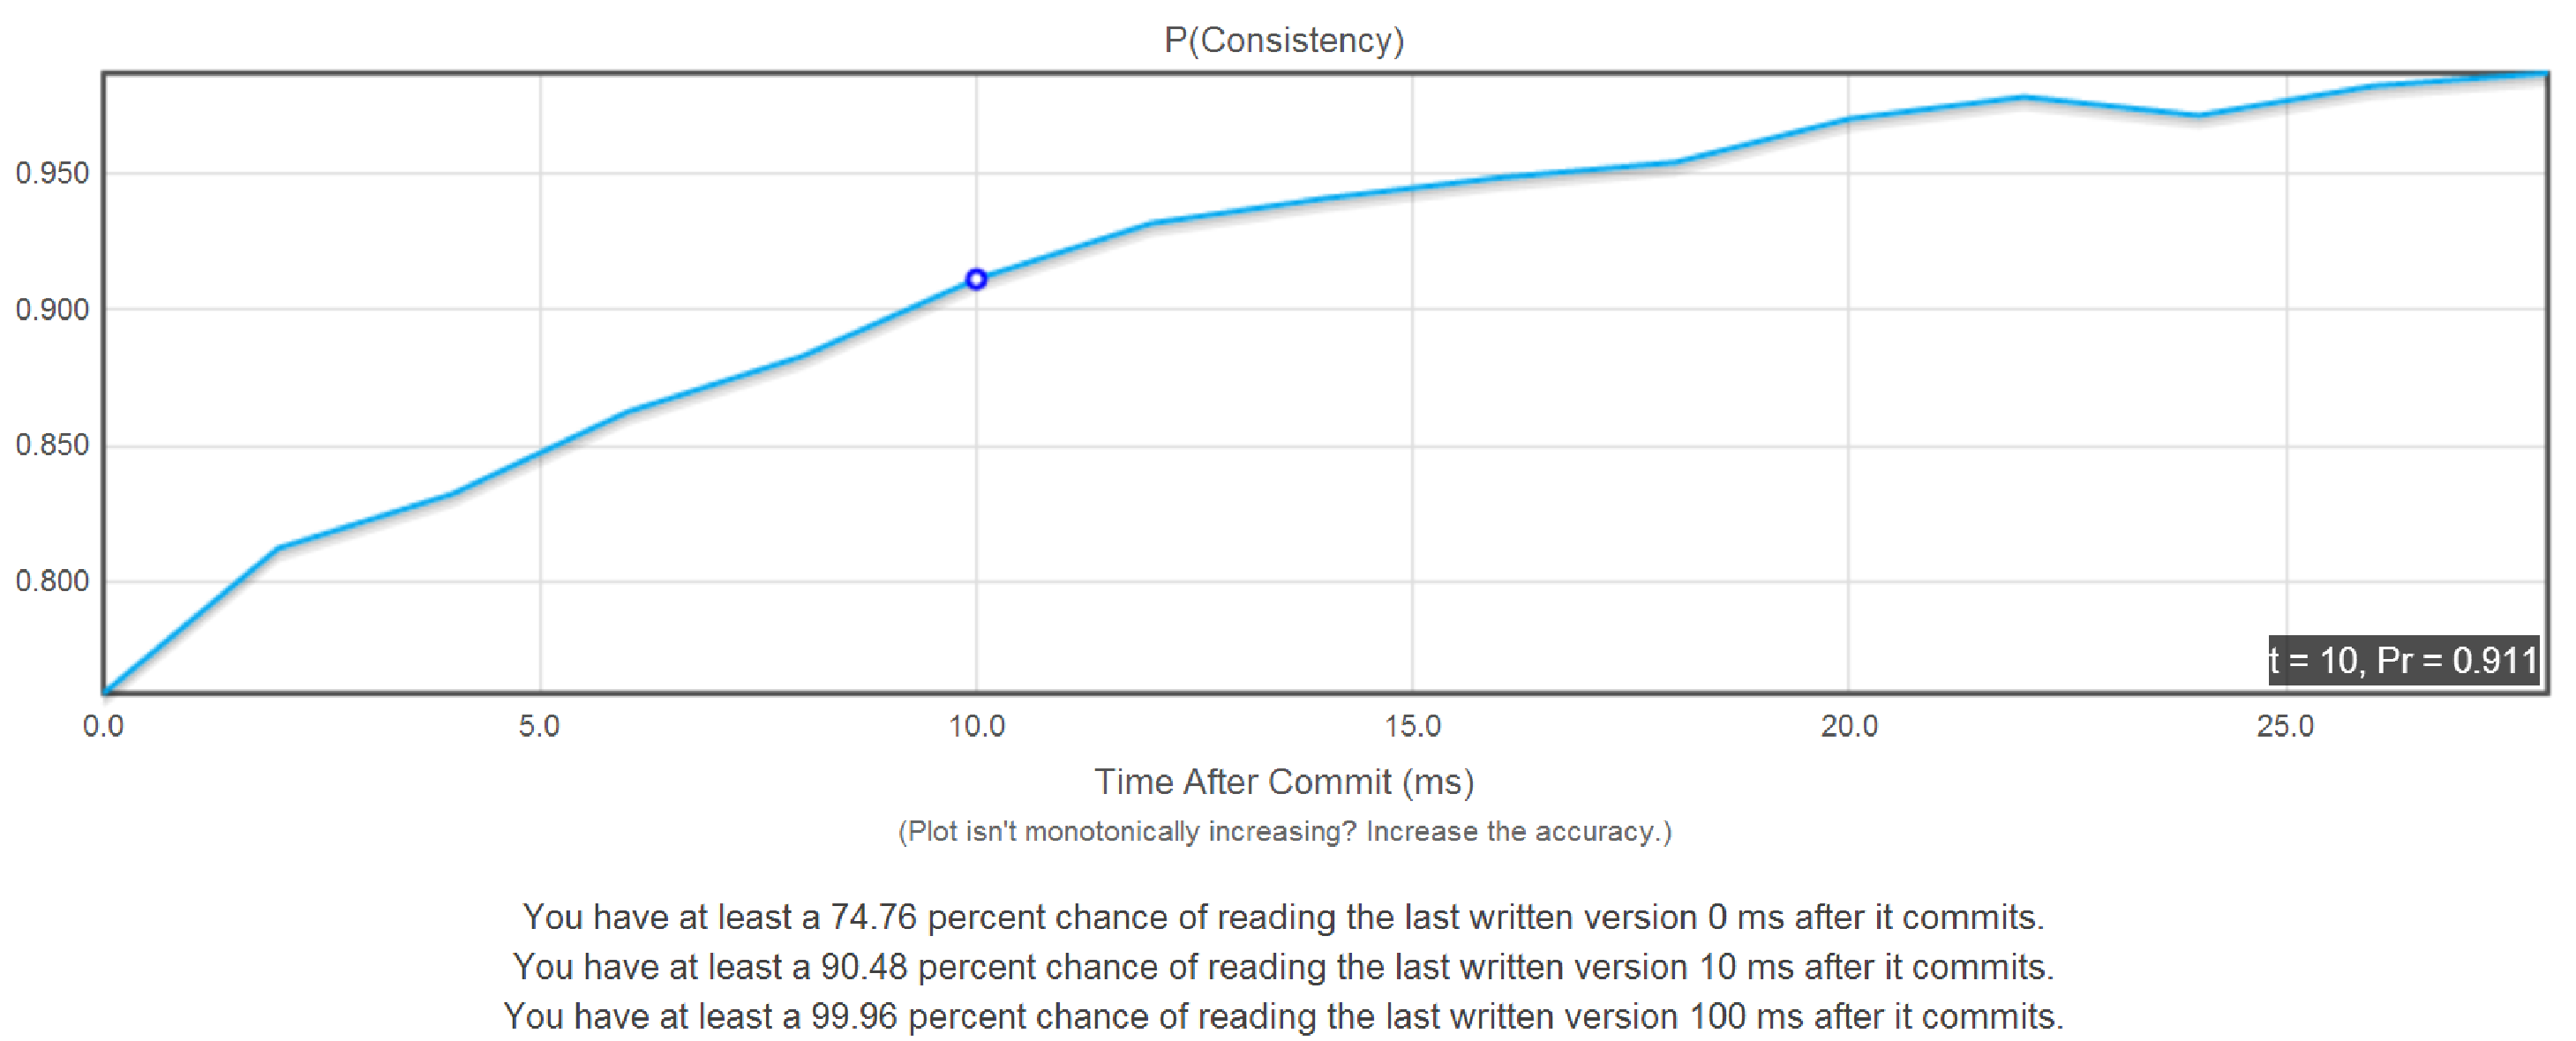
\includegraphics[width=.90\textwidth]{figs/pbs-demo-screenshot.pdf}
\subfigure[Mobile Web App]{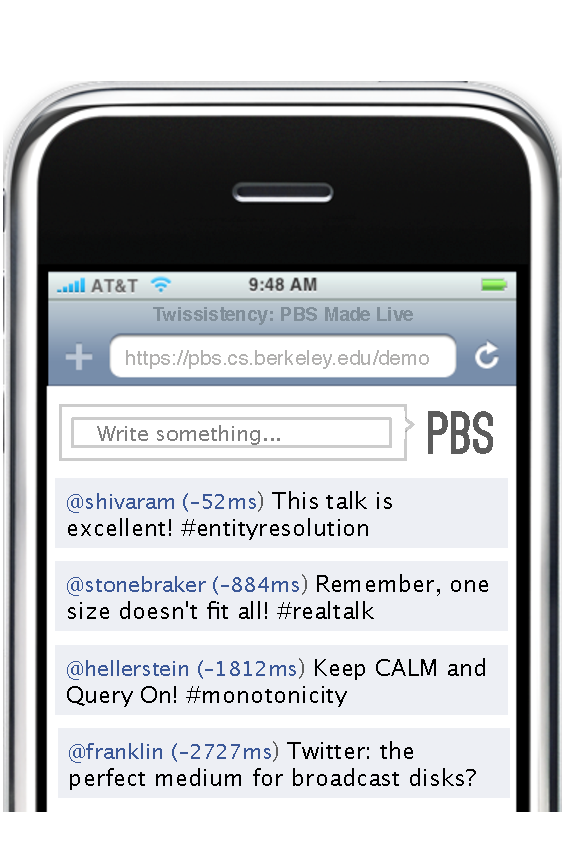
\includegraphics[width=.18\textwidth]{figs/phone.pdf}\label{fig:app}}
\hspace{0.12in}
\subfigure[DBA and Query Tuning Dashboard]{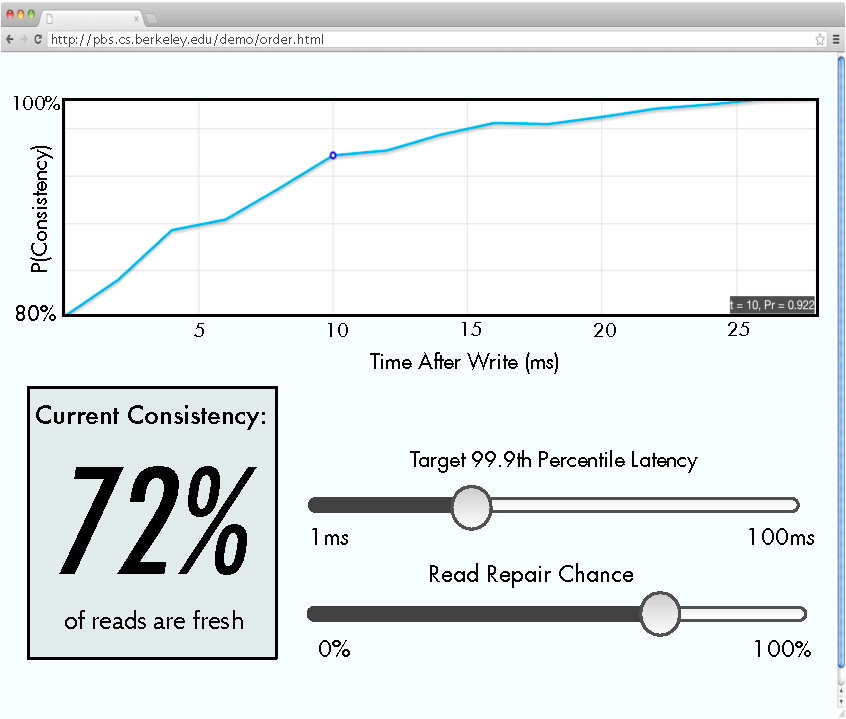
\includegraphics[width=.29\textwidth]{figs/dash.pdf}\label{fig:dash}}
\hspace{0.12in}
\subfigure[Chaos Console]{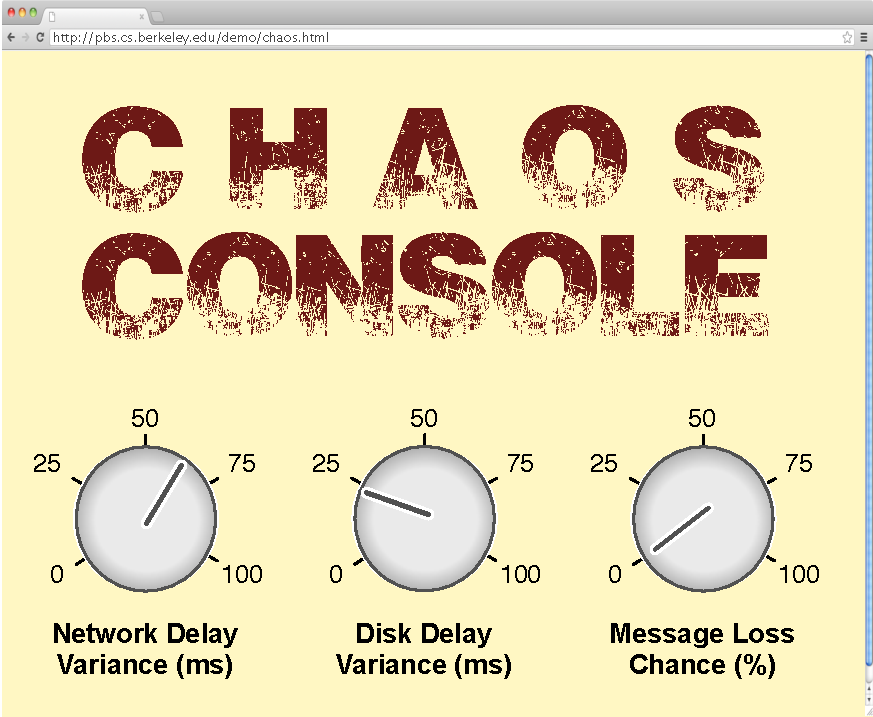
\includegraphics[width=.30\textwidth]{figs/chaos.pdf}\label{fig:chaos}}
\caption{Mock-ups for the mobile social web application---which
  attendees will interact with as end-users---and back-end diagnostic
  views. In the Dashboard, attendees can monitor system consistency
  and set latency and consistency SLAs. In the Chaos Console,
  attendees will wreak havoc on the application's Cassandra cluster
  via several (real-time) configurable failure modes.}
\label{fig:pbs-demo-screenshot}
\end{figure*}

\section{Demo details}
\label{sec:demo}
%Overall theme of the demo and what are goals are: Showing how PBS-metrics can be
%integrated into the DB admin's interface. Also showing why consistency metrics
%are important and how PBS can be used to measure this etc.

At SIGMOD 2013, we will present an end-to-end demonstration that will
show how metrics defined by PBS can be used to improve consistency and
user experience. We will also highlight how database administrators
can monitor and modify system parameters to trade-off consistency for
latency. The demonstration will consist of a user-facing application
and several other components.

%Specific demo setup details: What is the app going to be -- What tables is it
%going to contain and how is this stored in Cassandra ?

As a driving use case, we will implement \textbf{{\systemname}}, a
Twitter-like microblogging application. {\systemname} will expose a
web interface that will be available to all SIGMOD attendees and
provide a mobile application that can be used to post messages about
the conference. In addition to the messages posted by SIGMOD
attendees, we plan to \textbf{replay a corpus} of 4,937,001 Tweets
from conversations obtained from the Twitter firehose between February
and July 2011~\cite{ritter2010unsupervised}. This will help us explore
heavier workloads, particularly in the absence of a deluge of activity
from SIGMOD attendees. {\systemname} will store messages in a
\textbf{Cassandra cluster} running on Amazon EC2. PBS is already
integrated in Cassandra, but we will also augment Cassandra to provide
consistency monitoring as described in Section~\ref{sec:dbarch}.

%Demo screens detail - We will have two screens and what each one will show. How
%can the audience interact with the demo ?

To illustrate the utility of consistency metrics, we will provide
attendees with the opportunity to experience consistency from three
perspectives: user, administrator, and powerful adversary.

The \textbf{user interface} screen will host the {\systemname}
front-end and will allow attendees to post and read messages
(Figure~\ref{fig:app}). We will also provide a setting that
allows users to see how old messages are and manually inspect the
end-to-end delay for each message. %from the write to their chosen interface.

To provide the experience of a database administrator or operations
technician, we will have a \textbf{monitoring and control console}
that measures and plots the consistency and latency over 10-second
time intervals (Figure~\ref{fig:dash}).
%\footnote{We previously
%released an interactive, browser-based demo online at
%\url{http://pbs.cs.berkeley.edu/#demo} (but did not officially
%demonstrate it in a peer-reviewed forum). We expect to build a
%similar prototype for the first portion of the monitoring console
%design. However, the online demo is based on synthetic data, while
%the proposed demo runs in real-time on a real cluster.}
Additionally the interface will allow users to modify system parameters like
the read repair chance and set consistency SLAs for read and write
operations. We will change the system parameters in real-time, and the
consistency SLAs will affect all users' actions on the site
%---both from the replay stream and attendees accessing {\systemname}.

Consistency is particularly interesting under changing environmental
conditions, so we will allow participants to control parameters like
system latency and the performance of several replicas. We will provide
a \textbf{chaos console}, a separate interface that can be used to
inject message delays, model message loss, and artificially
slow Cassandra instances to demonstrate their effect on consistency
(Figure~\ref{fig:chaos}). We will physically implement the actual failures via
both JVM manipulation and host-based kernel operations. In addition to
improving engagement, this will allow attendees to both induce
consistency anomalies and understand the impact of several common
failure modes.

\balance
\section{High-level Takeaway}

This demo will demonstrate new data store performance and
administration functionality enabled by emerging consistency
prediction and monitoring. Given the amount of academic interest in
this topic and recent industrial adoption, we believe there is merit
in further study of applications that leverage these metrics. As a
proof-of-concept of several of the applications we envision, this
demonstration can serve as the impetus for a new wave of dynamic,
intelligent, and more easily operable distributed data
stores. Consistency metrics are coming; what else can we do with them?


\begin{comment}
\section{Acknowledgments}
We would like to thank Jonathan Ellis for his help in reviewing and integrating
our Cassandra patch.  WThank LinkedIn folks who helped in Voldemort measurement patch
etc.

This research is supported in part by NSF CISE Expeditions award CCF-1139158,
gifts from Amazon Web Services, Google, SAP,  Blue Goji, Cisco, Cloudera,
Ericsson, General Electric, Hewlett Packard, Huawei, Intel, Microsoft, NetApp,
Oracle, Quanta, Splunk, VMware and by DARPA (contract \#FA8650-11-C-7136).

TODO: Add any other funding agencies ?
\end{comment}


\bibliographystyle{abbrv}
\bibliography{pbs-demo}


\end{document}
